\documentclass[conference]{IEEEtran}
%\IEEEoverridecommandlockouts
% The preceding line is only needed to identify funding in the first footnote. If that is unneeded, please comment it out.
\usepackage{cite}
\usepackage{amsmath,amssymb,amsfonts}
\usepackage{algorithmic}
\usepackage{graphicx}
\usepackage{textcomp}
\usepackage{xcolor}
\usepackage{subcaption}
\def\BibTeX{{\rm B\kern-.05em{\sc i\kern-.025em b}\kern-.08em
    T\kern-.1667em\lower.7ex\hbox{E}\kern-.125emX}}
\begin{document}

\title{Kalman and Particle filter's robustness to non-linearity}

\author{
    \IEEEauthorblockN{Marius Oechslein}
    \IEEEauthorblockA{
        \textit{Faculty of Computer Science and Business Information Systems} \\
        \textit{University of Applied Sciences Würzburg-Schweinfurt}\\
        Würzburg, Germany \\
        marius.oechslein@study.thws.de
    }
        %\and
}
\maketitle

\begin{abstract}
The Kalman and the Particle filter are often used for estimating the real position of objects based on noisy observations.
% TODO: Maybe also investigate how kalman filter is affected?
In this paper we investigate how non-linearity, like the the impact of a thrown ball with a wall, can be modelled with the Kalman and Particle filter. \\
While the Kalman filter by definition is only applicable for linear systems, the Particle filter can also be used for non-linear systems.
Therefore it is interesting to explore how robust the Particle filter is for these kinds of non-linearities. \\
To investigate the robustness of the Particle filter to non-linearities, the Particle filter is first implemented with low variance and many observations.
This performance is then compared to an instance with a low amount of observations and an instance with high variance in the observations.
Since a low amount of observations and high variance is known to have a negative effect on the performance of the particle filter, it will be interesting to see whether the particle model can still model the non-linearity.
\end{abstract}

\begin{IEEEkeywords}
Particle Filter, Kalman Filter, Ball Throw, Boundary
\end{IEEEkeywords}

\section{Introduction}
The throw of a ball with noisy observations by a 2D camera can easily be modelled by a Kalman and Particle filter. 
Both the Kalman and the Particle filter are applicable for this problem due to the uncertainty in the noisy observations.
The Kalman filter by definition is able to model linear systems with high accuracy and the advantage of computationally cheap calculations. 
The Particle filter is also able to model such a problem by recursively estimating the most likely position of the ball over time. \\
In a non-linear system like the ball hitting a wall, which changes the direction of the ball, the Kalman filter can no longer model the systems dynamics.  
Although the Kalman filter tries to model the system dynamics as best as it can, it will not be able to model this non-linearity due to its basic assumptions. 
The Particle filter on the other hand is able to model such non-linearities. 
But it is interesting to investigate how robust the Particle filter is to such non-linearities like the ball changing its direction when hitting a wall. \\
To investigate this robustness the amount of observations is decreased and the variance of the observations are increased. 
The point of interest is if the Particle filter will still be able to model the non-linear direction change after the ball hits the wall.

% TODO: Irgendwo noch einen Absatz darüber, dass Particle filter das mit den drei Schritten ..., ... und ... rekursiv schafft, die Sachen zu modellen?

% TODO: 
%1. Establishing the research topic \\
%2. Establishing a niche \\
%3. Occupying the niche \\


\section{Physics of a ball throw}
% TODO: Sollte ich hier über die Physics schreiben? Ich glaube, ich könnte schon, wenn ich möchte.
The physics of throwing a ball have to be implemented in the state transition to be able to estimate the position of the ball in the next time step.  
The x-position can be modelled like this:
\begin{equation*}
    \begin{aligned}
    x_{t+1} = x_{t} + v_x * \Delta t,   \\
    x, v_x \in \mathbb{R}
    \end{aligned}
    \tag{1}
\end{equation*}
where the ${v_x}$ is the ball's constant velocity in x-direction and $x_t$ is the x-position of the ball at time step t. \\
The position and velocity in y-direction on the other hand are a bit more complex to calculate since they are affected by gravity.
\begin{equation*}
    \begin{aligned}
    y_{t+1} = y_t + v_y \Delta t - 0.5 g \Delta t^2, \\
    y, v_y \in \mathbb{R}
    \end{aligned}
    \tag{2}
\end{equation*}
with g being the gravity constant at $g = 9.81$. \\
When hitting a wall, the only change in the physical motions is that the velocity in x-direction has to be negated.
So at a after a certain time step where the wall is, the velocity in x-direction has to be updated to this $x^{vel} = -x^{vel}$.
The velocity in y-direction is unchanged with the assumption that there is no fraction when the ball hits the wall and that the wall is exactly vertical. 
The equation for the x-position also remains unchanged.


\section{Kalman and Particle filter}
In this section the Kalman and Particle filter are presented. 
% TODO: equations for the kalman and particles filters
For both the Kalman and Particle filter we define the hidden state as follows:
\begin{equation*}
\textbf{q} = (x, y, v_x, v_y)   \tag{3}
\end{equation*}
Only the x and y-positions are incorporated in the observations, given by
\begin{equation*}
    \begin{aligned}
    \textbf{o} = (x, y)
    \end{aligned}
\tag{4}
\end{equation*}

Both Kalman and Particle filters implement the following equation for the recursive density estimation:
\begin{equation*}
    p(\textbf{q}_t | \langle \textbf{o} \rangle _t) =
    p(\textbf{o}_t | \textbf{q}_t) \int p(\textbf{q}_t | \textbf{q}_{t-1}) p(\textbf{q}_{t-1} | \langle \textbf{q} \rangle _{t-1}) d \textbf{q}_{t-1}
\tag{5}
\end{equation*}

The Kalman filter does so by the Kalman gain algorithm \cite{b2}.
One important property of the Kalman filter is its linearity assumption.
Due to these assumptions non-linear systems cannot be modelled by the Kalman filter \cite{b2}. % TODO: Stimmt die Citation?
The Particle filter on the other hand can handle non-linearities and can be implemented by the Condensation algorithm \cite{b3}. \\
It was decided to only study the variance and the number of observations for the robustness, since the main point of interest was the direction change when the ball hit the wall.
Next to the variance and the number of observations, also the noise distribution and the starting assumed starting position has an effect on the robustness of the Particle filter.
Since the main interest of this paper is the impact with the wall, it was decided to only test the Particle filter on different values for the variance and the number of observations.
The noise was always assumed normally distributed and the starting positions were set to the real starting positions of the ball.

% TODO: Different Mathematical Notation ...
%\begin{figure}[h]
%\centerline{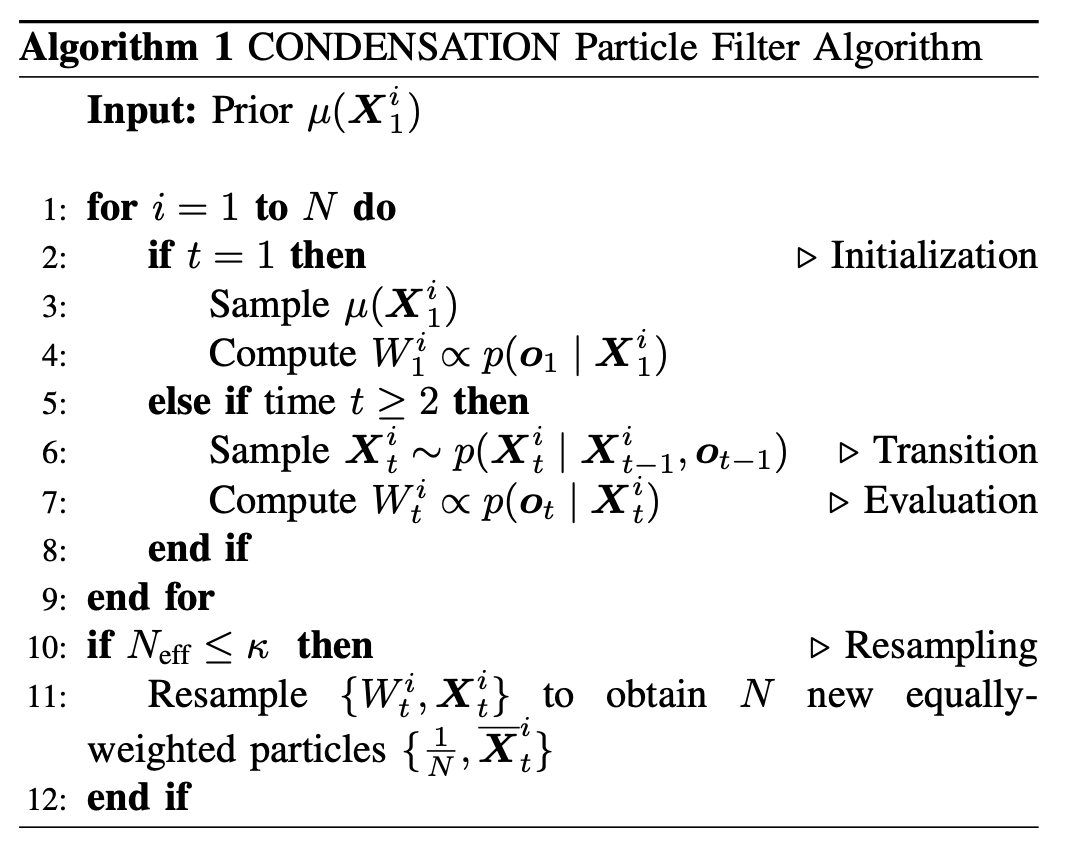
\includegraphics[width=70mm]{figs/condensation-algorithm.png}}
%\caption{Condensation Particle filter algorithm from \cite{b1}.}
%\label{fig:condensation-algorithm}
%\end{figure}


% Structure:
%0. Physics of ball. Also using it for the state transition model later. \\
%1. Simple Math Notations used for Kalman filter \\
%2. Simple Math Notations usef for Particle Filter \\
%3. Somehow introducing the boundaries to Particle Filter math? \\


\section{Results}

% TODO:
% TODO: For all: make sure if it is variance or Standard deviation!

% Kalman filter with time_sim=5, time_step=0.1, variance=1
% Particle filter 1 boundary normal: time=5, time_step=0.1, variance=1
% Particle filter 1 boundary high variance: time=5, time_step=0.1, variance=8 -> 50 observations
% Particle filter 1 boundary few observations: time=5, time_step=0.1, variance=1 -> 12 observations
% Kalman filter 3 boundaries: time_sim=5, time_step=0.1, variance=1
% Particle filter 3 boundaries normal: time=5, time_step=0.025, variance=0.5 -> 200 observations! and lower variance
% Particle filter 3 boundaries higher variance: time=5, time_step=0.025, variance=1 -> way worse for only a little bit more noise
% Particle filter 3 boundaries fewer observations: time=5, time_step=0.1, variance=0.5 -> 50 observations

% Ich muss aufpassen, dass ich nicht zu viele Plots zeige. 
% Der Vergleich von Robustness of 1 boundary zu 3 boundaries ist aber trotzdem interessant!
% Vielleicht nur auf few observations ODER high variance konzentrieren und dabei 1 boundary neben 3 boundaries plotten und deren Metrics vergleichen
% Dabei ist es aber wichtig, dass die restlichen Parameter gleich bleiben -> Dann sieht man sofort, dass multiple boundaries viel anfälliger ist als 1 boundary.
% -> These ist also: Nimmt die robustness ab, wenn der throw mit boundaries more complex wird, bzw. more non-linearities. !!!

\subsection{Kalman and Particle Filter modelling non-linearities} % Do I need this? Only need this, when I include the second \subsection

First the results of the Kalman filter for estimating the positions of the ball are shown.   
\begin{figure}
	\centering
	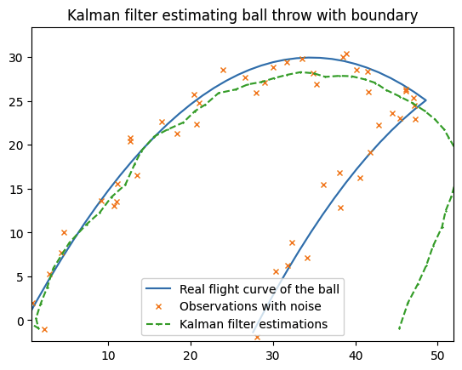
\includegraphics[width=70mm]{figs/kalman-filter.png}
	\caption{Kalman filter modelling non-linearities. From own calculations.}
	\label{fig:kalman-filter}
\end{figure}
The Kalman filter behaves as expected by not being able to model the non-linearities well.
Since the Kalman filter is already not able to model one non-linearity, its performance is likely to decrease as the complexity increases.
The robustness of the Kalman filter to non-linearities is already known \cite{}, therefore any further experiments concerning robustness of the Kalman filter are uninteresting. \\
For the rest of this section, we focus on the robustness of the Particle filter as the non-linearity increases. 
% TODO: Is this the correct place for this, or should I move it to the Methods section?
To compare the robustness of Particle Filter for the cases of one non-linearity and multiple non-linearities, we investigate each of the cases seperately while changing parameters that test the robustness of the method. 
For both the one non-linearity and the multiple non-linearities, the Particle Filter is first tested on reasonable values for the variance of and the number of observations. 
After that the variance and the number of observations are changed in order to test the robustness of the Particle filter. 
\begin{figure}
	\centering
	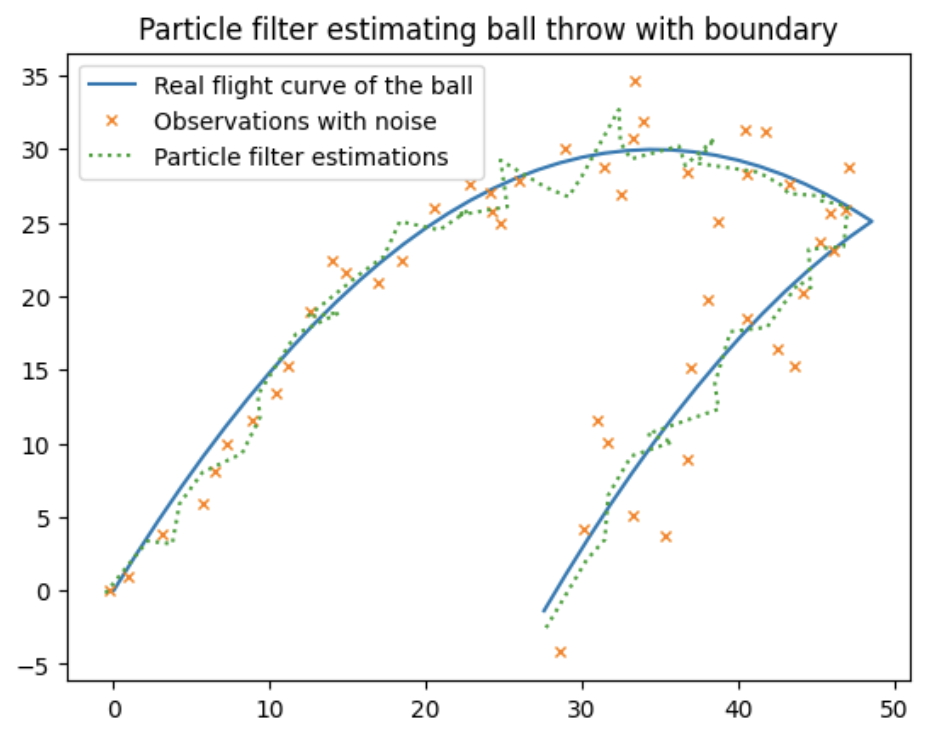
\includegraphics[width=70mm]{figs/particle-filter-one-boundary}
	\caption{Particle filter with one boundary. From own calculations.}
	\label{fig:particle-filter-one-boundary}
\end{figure}
\begin{figure}
	\centering
	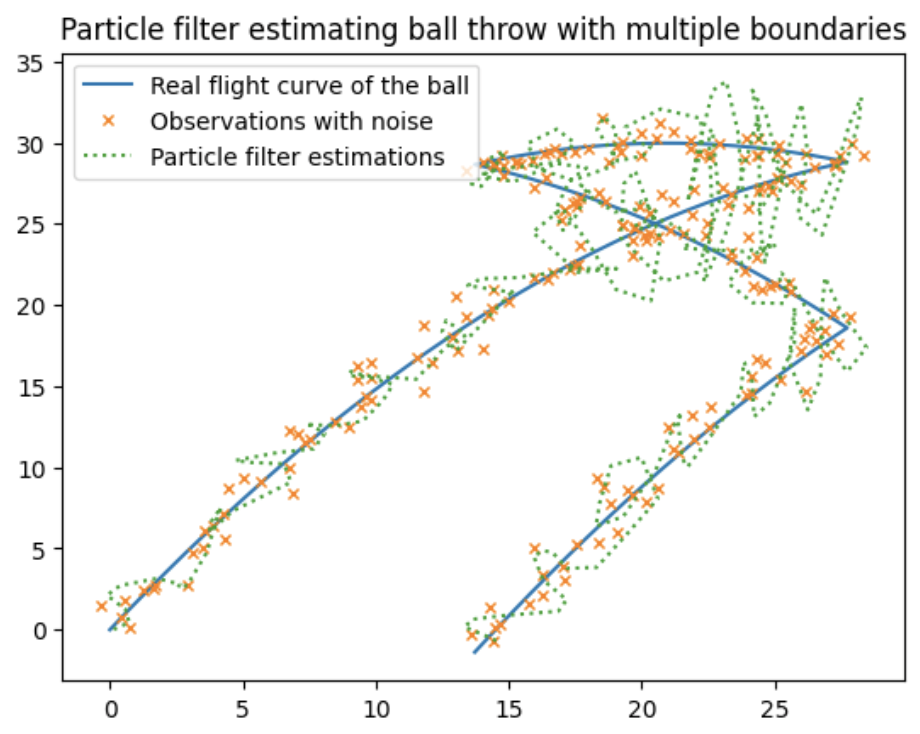
\includegraphics[width=70mm]{figs/particle-filter-multiple-boundaries}
	\caption{Particle filter with multiple boundaries. From own calculations.}
	\label{fig:particle-filter-multiple-boundaries}
\end{figure}
Note that the variance and the number of observations had to be decreased substantially when increasing the number of non-linearities. 
This already indicates that the Particle filter struggles more to model the ball throw as the number of non-linearities increase. 
For fig. \ref{fig:particle-filter-one-boundary} the variance of the noise is set to 1 and the number of observations are set to 50.
For fig. \ref{fig:particle-filter-multiple-boundaries} on the other hand, the variance for the noise had to be changed to 0.025 and the number of observations had to be increased to 200 for the Particle filter to model the ball throws reasonably well. \\

\begin{table}[htbp]
    \caption{Estimation errors for one boundary. Boundary 50 m away.}
    \begin{center}
    \begin{tabular}{|c|c|c|}
    \cline{1-3}
    & Before hitting the wall & After hitting the wall \\
    \cline{1-3} 
    Kalman filter & \textit{1.2 m} & \textit{17.73 m} \\
    \cline{1-3} 
    Particle filter & \textit{1.87 m} & \textit{3.01 m} \\
    \hline
    \end{tabular}
    \label{tab:comparing-kalman-particle}
    \end{center}
\end{table}
The errors of estimation for the Kalman and Particle filter both increase as the ball hits the wall \ref{tab:comparing-kalman-particle}.
But the Particle filter is able to estimate the position much better after this non-linearity.
Before the ball hits the wall the Kalman filter is around 0.5 m more accurate than the Particle filter, but this difference could be partly due to the uncertainty of the observations and the Particle filter.
% TODO: Hier mehr schreiben? Mehr vergleichen?


\subsection{Testing the robustness of the Particle filter}
In this section the robustness of the Particle filter is further tested for the case of multiple boundaries.
First the variance of the noise is increased from 0.025 to 1.
\begin{figure}
	\centering
	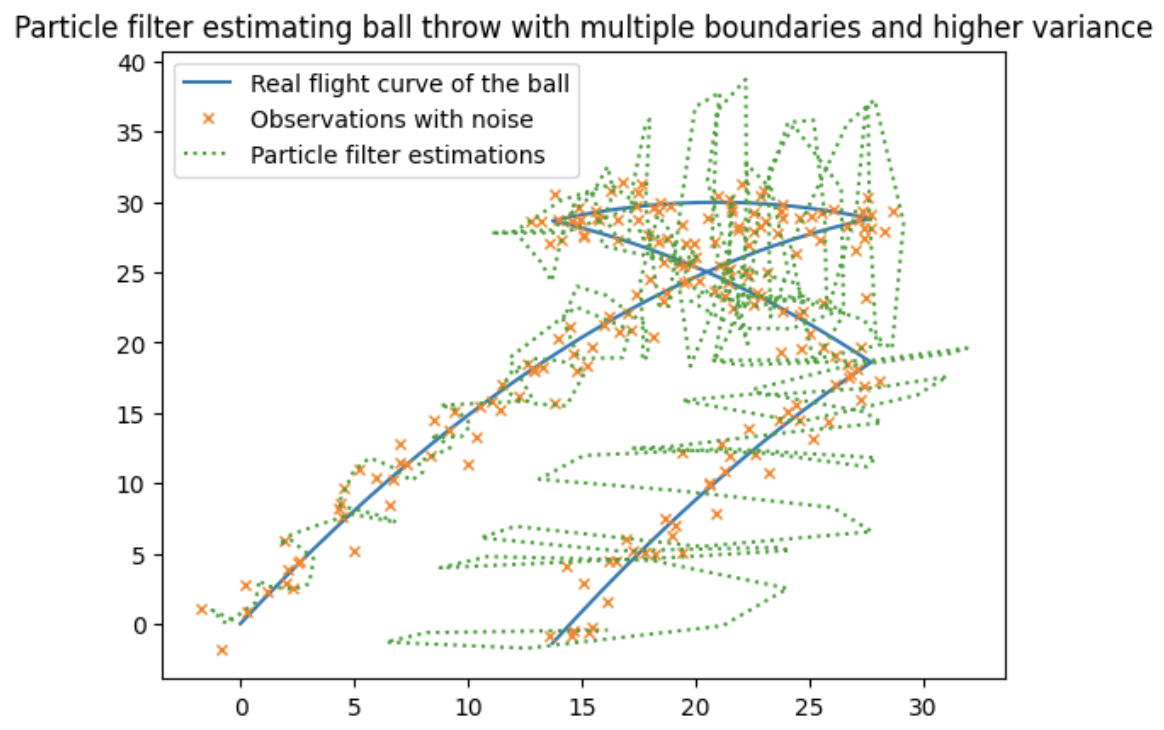
\includegraphics[width=70mm]{figs/particle-filter-multiple-boundaries-higher-variance}
	\caption{Particle filter with multiple boundaries and higher variance. From own calculations.}
	\label{fig:particle-filter-multiple-boundaries-higher-variance}
\end{figure}

Note that this is the same variance that was used for the Particle filter with one boundary in fig. \ref{fig:particle-filter-one-boundary}.
Since this estimation in fig. \ref{fig:particle-filter-multiple-boundaries-higher-variance} is much worse than for the Particle filter with one boundary with the same variance for the noise, it indicates that the robustness of the Particle filter decreases as the number of non-linearities increase. 
\begin{figure}
	\centering
	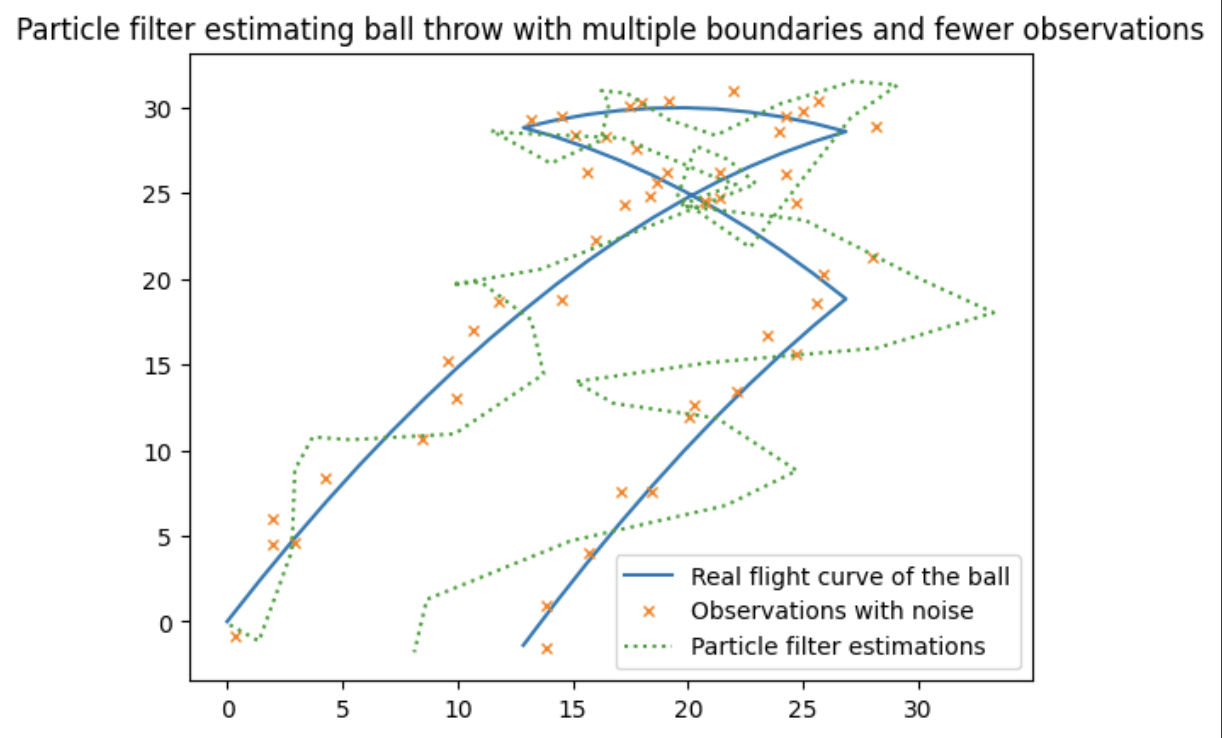
\includegraphics[width=70mm]{figs/particle-filter-multiple-boundaries-fewer-observations}
	\caption{Particle filter with multiple boundaries and fewer observations. From own calculations.}
	\label{fig:particle-filter-multiple-boundaries-fewer-observations}
\end{figure}

Decreasing the number of observations in fig. \ref{fig:particle-filter-multiple-boundaries-fewer-observations} also results in a worse estimation.
Also note here that this is the same number of observations as in fig. \ref{fig:particle-filter-one-boundary} for the Particle filter with one boundary.

\begin{table}[htbp]
    \caption{Estimation errors for multiple boundaries. First boundary 25 m away.}
    \begin{center}
    \begin{tabular}{|c|c|c|}
    \cline{1-3}
		Before (fig. \ref{fig:particle-filter-multiple-boundaries}) & Higher variance (fig. \ref{}) & Fewer observations (fig. \ref{}) \\ % TODO: How should I name these
    \cline{1-3} 
		\textit{TODO m} & \textit{TODO m} & \textit{TODO m} \\
    \hline
    \end{tabular}
    \label{tab:comparing-kalman-particle}
    \end{center}
\end{table}

In conclusion comparing the results of the Particle filter for one boundary (fig. \ref{fig:particle-filter-one-boundary}) and multiple boundaries (fig. \ref{fig:particle-filter-mulitple-boundaries}) indicate that the robustness of the particle filter decreases as the number of non-linearities increase.
The experiments of changing the variance (fig. \ref{fig:particle-filter-multiple-boundaries-higher-variance}) and the number of observations (fig. \ref{fig:particle-filter-multiple-boundaries-fewer-observations}) indicate the same relation.  


%1. Result of kalman filter handling the boundary \\
%2. Result of Particle filter handling the boundary with "known system dynamics" for the state transition \\
%3. Result of Particle filter handling the boundary without knowing the system dynamics/ knowing of the boundary \\

\section{Discussion}

% TODO:
% Particle degeneracy, Smoothing performance, ...
% These are the popular problems of Particle filter
% I can get them from comparing the normal Particle filter with advanced ones and see which problems the advanced ones solve
% Also I can see some of the problems in his slides


%1. We see that the kalman filter is not able to apply for this "non-linear" problem. Because Kalman filter expects linear relations. Maybe an advanced Kalman filter would be applicable. \\

\section{Conclusion}

It would be interesting to see whether an advanced form of the kalman filter would be able to handle this non-linearity. 
- Naming which kind of kalman filter would be able to do it probably.
Other than that we could look at the particle filter not knowing the system dynamics in the state transition (like not knowing of the boundary in the state transition).




\section*{References}

Please number citations consecutively within brackets \cite{b1}. The 
sentence punctuation follows the bracket \cite{b2}. Refer simply to the reference 
number, as in \cite{b3}---do not use ``Ref. \cite{b3}'' or ``reference \cite{b3}'' except at 

\begin{thebibliography}{00} % TODO
\bibitem{b1} Fetzer, T., Bullmann, M., Ebner, M., Kastner, S., Deinzer, F., \& Grzegorzek, M. Interacting Multiple Model Particle Filter for Indoor Positioning Applications.
\bibitem{b2} Thrun, S. (2002). Probabilistic robotics. Communications of the ACM, 45(3), 52-57. % TODO: Correct?
\bibitem{b3} Isard, M., \& Blake, A. (1998). CONDENSATION--conditional density propagation for visual tracking. International journal of computer vision, 29(1), 5.
    
%\bibitem{b1} G. Eason, B. Noble, and I. N. Sneddon, ``On certain integrals of Lipschitz-Hankel type involving products of Bessel functions,'' Phil. Trans. Roy. Soc. London, vol. A247, pp. 529--551, April 1955.
\end{thebibliography}

\end{document}
